% begin module transformations-shifts
\begin{frame}
\frametitle{Transformations of Functions}
\begin{columns}[c]
\column{.5\textwidth}

\psset{xunit=1cm, yunit=1cm}
\begin{pspicture}(-0.5, -0.5)(4.7,4.7)%
\tiny%
\psframe*[linecolor=white](-5,-5)(5,5)%
\psaxes[ticks=none, labels=none]{<->}(0,0)(-0.5,-0.5)(5,4.5)%
\rput[t](5, -0.1){$x$}%
\rput[r](-0.1, 4.5){$y$}%
%\frac{1}{3} (3 x-6)^{3}-\frac{1}{3} (3 x-6)^{2}-\frac{1}{3} x+\frac{8}{3} 
\newcommand{\theFun}{3 x mul 6 sub dup dup mul mul 3 div 3 x mul 6 sub dup mul -3 div x -3 div 8 3 div add add add\space}%
\only<handout:0| -2>{%
\psplot[linecolor=red, plotpoints=1000]{1.65}{2.55}{\theFun}%
\rput[b] (2.55, 2.40654){\alert<-2>{$y=f(x)$}}%
}%
\only<handout:1| 3->{%
\psplot[linecolor=blue, plotpoints=1000]{1.65}{2.55}{\theFun}%
\rput[b] (2.55, 2.40654){$y=f(x)$}%
}%
\only<handout:0| 3>{%
\psplot[linecolor=red, plotpoints=1000]{1.65}{2.55}{\theFun 1.5 add }%
\rput[b](2.55, 3.90654){\alert<3>{$y=f(x)+c$}}%
}%
\only<handout:1| 4,5,22->{%
\psplot[linecolor=blue, plotpoints=1000]{1.65}{2.55}{\theFun 1.5 add }%
\rput[b](2.55, 3.90654){$y=f(x)+c$}%
}%
\only<handout:0| 4>{%
\psplot[linecolor=red, plotpoints=1000]{1.65}{2.55}{\theFun 1.5 sub}%
\rput[b](2.55, 0.906542){$y=f(x)-c$}%
}%
\only<handout:1| 5,22->{%
\psplot[linecolor=blue, plotpoints=1000]{1.65}{2.55}{\theFun 1.5 sub}%
\rput[b](2.55, 0.906542){$y=f(x)-c$}%
}%
\only<handout:0| 19>{%
\psplot[linecolor=red, plotpoints=1000]{3.15}{4.05}{1 dict begin /x x 1.5 sub def \theFun end}%
}%
\only<handout:1| 20,22->{%
\psplot[linecolor=blue, plotpoints=1000]{3.15}{4.05}{1 dict begin /x x 1.5 sub def \theFun end}%
\rput[b](4.05, 2.40654){$\alert<20>{y=f(x-c)}$}%
}%
\newcommand{\theAnimation}[6]{%
\uncover<handout:0|####1>{%
\fcXTickWithLabel{\curPt}{$x$}%
}%
\uncover<handout:0|####2>{%
\fcXTickWithLabel{\curPt 1.5 sub}{$x-c$}%
}%
\uncover<handout:0|####3>{%
\rput[l](! \curPt 1.5 sub 0.1 add 1 dict begin /x \curPt 1.5 sub def \theFun  end 2 div){$f(x-c)$}%
}%
\uncover<handout:0|####4>{%
\psline[linecolor=red, linewidth=2pt](! \curPt 1.5 sub 0)(! \curPt 1.5 sub 1 dict begin /x \curPt 1.5 sub def \theFun  end)%
}%
\uncover<handout:0|####5>{%
\rput[l](! \curPt 0.1 add 1 dict begin /x \curPt 1.5 sub def \theFun  end 2 div){$f(x-c)$}%
}%
\uncover<handout:0|####6>{%
\psline[linecolor=red, linewidth=2pt](! \curPt 0)(! \curPt 1 dict begin /x \curPt 1.5 sub def \theFun  end)%
}%
}%
\newcommand{\curPt}{3.3\space}%
\theAnimation{7-10}{8-10}{9-10}{9-19}{10}{10-19}%
\renewcommand{\curPt}{3.5\space}%
\theAnimation{11-14}{12-14}{13-14}{13-19}{14}{14-19}%
\renewcommand{\curPt}{3.8\space}%
\theAnimation{15-19}{16-19}{17-18}{17-19}{18}{18-19}%
%

\only<handout:0|21>{%
\psplot[linecolor=red, plotpoints=1000]{0.15}{1.05}{1 dict begin /x x 1.5 add def \theFun end}
\rput[b](1.05, 2.40654){\alert<6>{$y=f(x+c)$}}
}
\only<handout:1|22->{%
\psplot[linecolor=blue, plotpoints=1000]{0.15}{1.05}{1 dict begin /x x 1.5 add def \theFun end}
\rput[b](1.05, 2.40654){$y=f(x+c)$}
}
\end{pspicture}
%\ \only<handout:0| -2>{%
%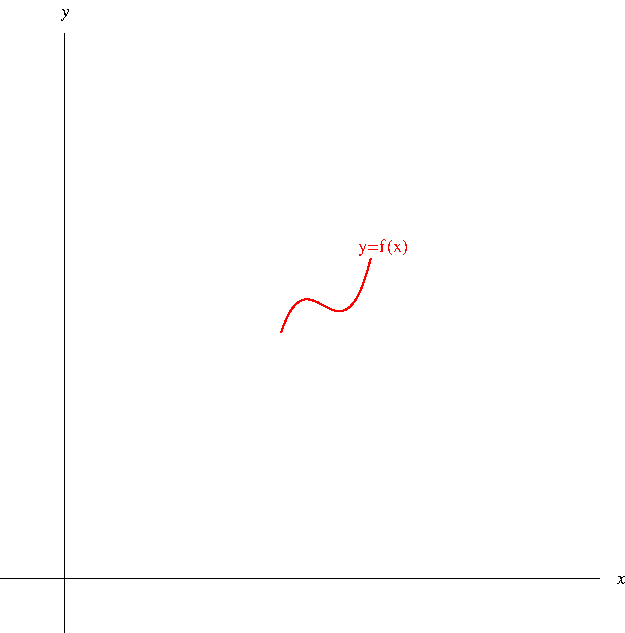
\includegraphics[height=5cm]{precalculus/pictures/01-03-shifta.pdf}%
%}%
%\only<handout:0| 3>{%
%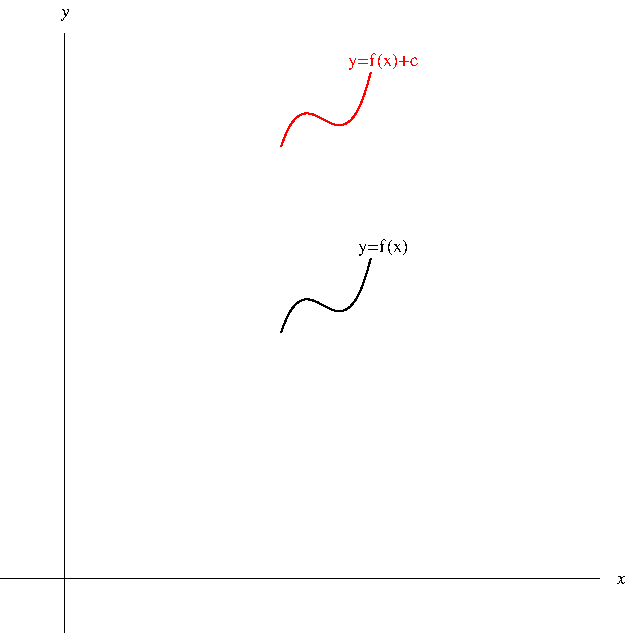
\includegraphics[height=5cm]{precalculus/pictures/01-03-shiftb.pdf}%
%}%
%\only<handout:0| 4>{%
%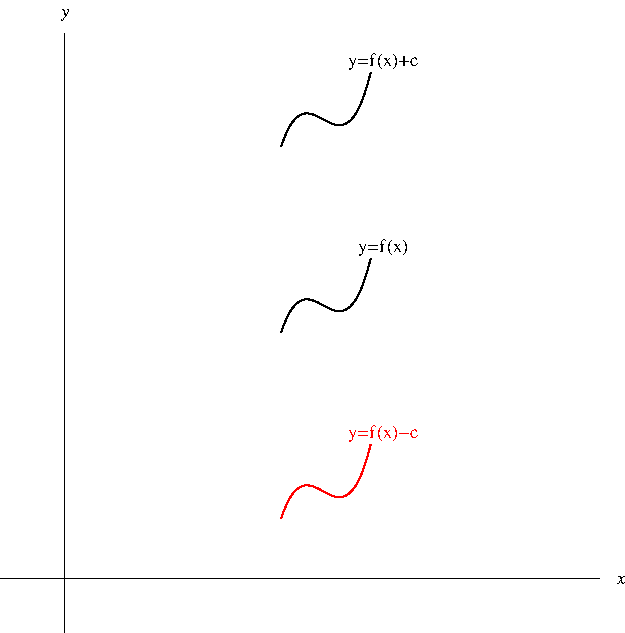
\includegraphics[height=5cm]{precalculus/pictures/01-03-shiftc.pdf}%
%}%
%\only<handout:0| 5>{%
%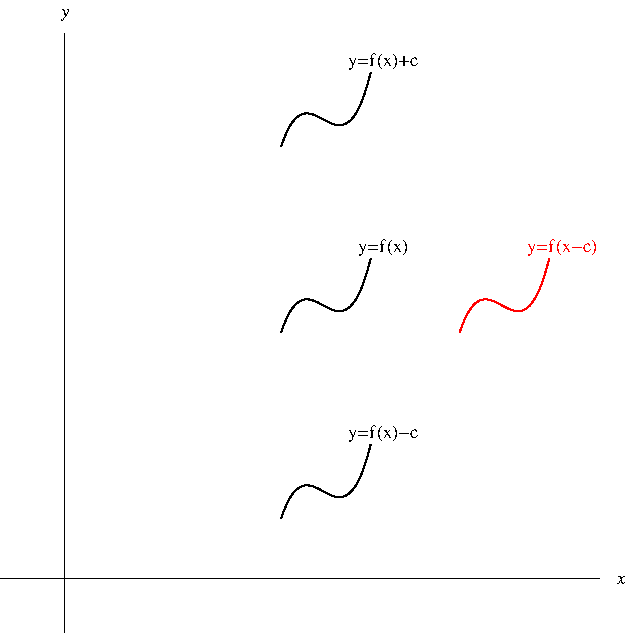
\includegraphics[height=5cm]{precalculus/pictures/01-03-shiftd.pdf}%
%}%
%\only<6>{%
%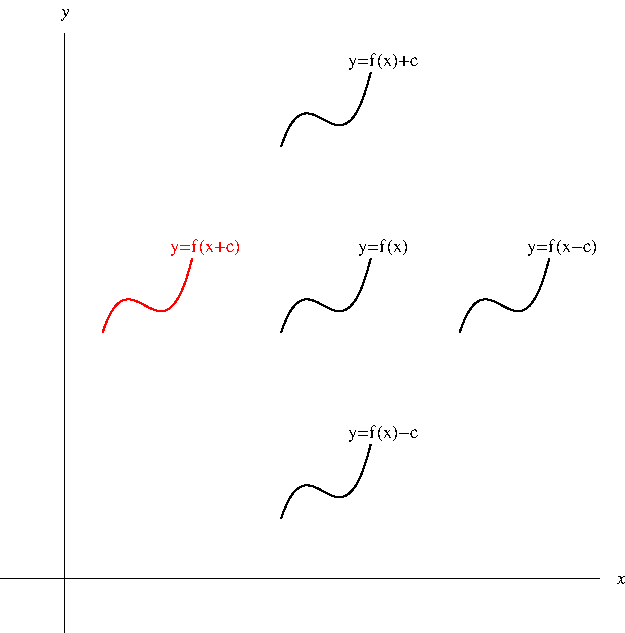
\includegraphics[height=5cm]{precalculus/pictures/01-03-shifte.pdf}%
%}%a
\column{.5\textwidth}
\begin{itemize}
\item What happens to the graph if we add/subtract a positive constant $c$ in the equation of a function $f$?
\item What happens if we add or subtract $c$ from $x$ before applying the function $f$?
\end{itemize}
\end{columns}

\uncover<2->{
\begin{tabular}{|l|l|}
\hline
\alertNoH{ 3}{$f(x)+c$} &%
\uncover<3->{\alertNoH{3,22}{Shift the graph of $f(x)$ $c$ units up.}} \\%
\alertNoH{ 4}{$f(x)-c$} &%
\uncover<4->{\alertNoH{4,22}{Shift the graph of $f(x)$ $c$ units down.}} \\%
\alertNoH{6}{$f(x-c)$} &%
\uncover<6->{\alertNoH{6,22}{Shift the graph of $f(x)$ \fcAnswerUncover{6}{20}{$c$ units right}.}} \\%
\alertNoH{21}{$f(x+c)$} &%
\uncover<21->{\alertNoH{21,22}{Shift the graph of $f(x)$ $c$ units left.}}\\%
\hline
\end{tabular}

}
\end{frame}
% end module transformations-shifts
